%----------------------------------------------------------------------------
\chapter{Részletes megvalósítás}
\label{sec:Details}
%----------------------------------------------------------------------------

Ebben a fejezetben a korábban röviden bemutatott építőelemekről adok egy részletsebb leírást.
Bemutatom, hogy az én projektemben milyen megoldásokat valósítottam meg a használatukkal.
Ahol van értelme diagramokon keresztül mutatom be a működését, ami látványos azt képekkel is illsóusztrálom.
Több kódrészet is szerepelni fog a fejezetben amiknek célja a kód működésének jobb mégétése.

\section{Compose}
\label{sec:Compose}

A Composeról korában már adtam egy átfogó leírást a \refstruc{sec:JetpackCompose}ban, most ebben a részben részleesebben bemutatom az alapaeleveket, használtatát és a keletekező képernyőket.

\subsection{Compose alapelvek, használata valós környezeteben}

Mivel a Compose egy deklreatív UI kit ezért összefoglalnám a legfontosabb részeit.
A UI elmeket nem lehet lehet direktben példányosítani, és kódból később elérni és ezen a referncián eresztül módosítani a tulajdonságait.
Minden egyes elem egy függvényhívást jelent, az állapotát és tulajdonságait pedig ezen belül lehet szábályozni és bállítani egyéb objektumokon és stateken keresztül.
Ezeket az állapotokat általában nem a Composable függvéyne belül tároljuk hanem egy ViewModelben, mivel az tartósabb. (\refstruc{fig:ViewModel})
Egy figyelt állapot hatására meghívódik a recomposoition, azaz a függvény újra meghívódik és frissíti a UI állapotát.
Az általános elv az, hogy egy Composable függvény nagy betűvel kezdődik, és attól lesz egy függvéyn Composable, hogy elé helyezzük a @Composable anntotációt.

Mi is az a recomposoition?
Röviden valamilyen állapotváltozást követő újra kirajzolódás.
Gyakran valamilyen felhasználói interakció váltja ki (gomb megnyomása, görgetés), de a ViewModelből is jöhet ez a változás (megérkezik a kezdeti adat, folyamotson frissülő információk jönnek), de okozhatja egy animáció is.

A Compose hasznátának van 5 fontos alapszáblya amelyek betartásával nem csak helyes, de gyors és dinamikus frissülő képernyőket tudunk egyszerűen létrehozni.
\begin{enumerate}
    \item A Composable függvények bármilyen sorrendben végrehajthatók.
    \item A Composable függvények párhuzamosan hajthatók végre.
    \item A Recomposition kihagyja a lehető legtöbb Composable függvényt és lambdát.
    \item A Recomposition optimista, és leállítható menet közben.
    \item Egy Composable függvény nagyon gyakran is futhat/ismétlődhet, olyan gyakran is, mint egy animáció minden képkockája.
\end{enumerate}

Pontosan mit is jelentenek ezek a szabályok?
Az 1. és 2. pont alapján következik, hogy minden Composable függvény önálló legyen, nem függhet egy másik Composable függvénytől sem.
Továbbá fontos, hogy ha ugyan azon stateet változtatják akkor az ne fusson le minden recomposoition során, ha ezt nem tartjuk be akkor folyamoatosn újra kirajzolódik a képernyő és lefagy az eszköz.
A 3. pont értelmezése, hogy csak a szükséges és részek renderelődnek újra, ezzel gyorsítva a folyamatot. Így amennyiben több függvényt is meghívnk egy másikon belül csak azok fognak újra rajzolódni amik függnek a változott állapottól.
Elő fordulhat, hogy mindent szeretnénk újra firissíteni, vagy több függvényt ami nem függ tőle, ehez használhatunk az állapottól függő Launched effectet vagy átadhatjuk az állaptot ezekenk a függvényknek is, és ott sinálhatumk vele egy egyszerű és gyors műveletet.
A 4. és 5. pont összefügg, ha új állapot érkezik és nem fejeződött be a recomposoition akkor előrről kedzi a folyamatot. Ne itt hajtsunk végre egy hosszú műveletet (HTTP kérések indítása), ez feleslges overheadet jelent mert senki nem állítja le az aszinkron hívást, és nem is tud hova visszaérkezni az adat így feleslgesen használtuk az erőforrsáokat mind a két oldalon.
Ne állítsunk be egy olyan értéet sem itt amire szükségünk lehet később, mivel nem biztos, hogy eljut a futás addig vagy, lehet, hogy a következő másodpercben már felül lett írva mással.

Az alábbi kódrészetben bemutatom, hogy milyen részekből tevődik össze egy Composable függvény.
\begin{lstlisting}[caption={Composable függvény részei.}, label={lst:ComposableParts}, language=Kotlin]
@Composable     // A kötelező annotáció
fun ExamEditResultScreen(   // Függvényparaméterek
    navigateBack: () -> Unit,       // Egy lambda függvény fejléce
    viewModel: ExamEditViewModel,   // ViewModel átadása paraméterként
    modifier: Modifier = Modifier   // Modifier amivel a kinézetet lehet testre szabdni.
) {
    val coroutineScope = rememberCoroutineScope()           // Coroutine scope lekérése, így lambda függényben használható, mivel annak a törzse nem Composable függvény.
    var showNotify by remember { mutableStateOf(false) }    // Statek amit el lehet tárolni a Composable függvényben mivel ezen kívül nincs használva.
    var notifyMessage by remember { mutableStateOf("") }    // Statek amit el lehet tárolni a Composable függvényben mivel ezen kívül nincs használva.
    if (showNotify) { Notify(notifyMessage); showNotify = false} // Állapottól függő megjelenítés
    Scaffold(   // Beépített Composable elem amivel egy általános Android nézetet könnyen létre lehet hozni.
        topBar = { TopAppBarContent(stringResource(Res.string.exam_edit), navigateBack) },  // Itt egy topBart lehet könnyen megadni.
    ){innerPadding ->   // Ez a belső része a képenyőnek, a fő része az alkalmazásnak.
        ExamEntryBody(      // Egy másik Composable elem meghívása, ami a megjelnésért felel.
            examUiState = viewModel.examUiState,           // Szüksége van viewModelben lévő statere
            onExamValueChange = viewModel::updateUiState,  // Nevesített függvényt így lehet átadni egy lambda függvénynek
            onSaveClick = {     // Lambda függvényt helyben is megadhatunk
                coroutineScope.launch { // Itt látható egy példa a trailing lambda használatára
                    if(viewModel.updateExam()){ navigateBack() }    // If-else szerkezet is nyugodtan használhatunk. Siker esetén visszanavigál
                    else{   // Egyéként a sikerttelenséget közli a felhasználóval
                        showNotify = true
                        notifyMessage =  "Exam with this name already exists"
                    }
                }
            },
            modifier = modifier.padding(innerPadding))}}
\end{lstlisting}

\subsection{Alkalmazás bemutatása képernyőképekkel}

Ebben az alfejezetben bemutatom az elkészült képernyőket és a hozzájuk tartozó érdekes részeket, megoldásokat.

\subsubsection{A fő képernyők}

A két alkalamzás típusra más-más a felhasználói igény.
Androidon, ahol általában egy álló képernyő van (\refstruc{fig:MainScreen} jobb oldal) és a telefont a jobb alsó sarokban fogjuk meg nem esik kézre a fent bekapcsolható menü (bár oldalra huzással is előhozható). 
Asztali alaklamzás estén viszont jobban mutat ez a megoláds, és egy nagyobb képernyő ahol a kiválasztott funkció képernyője meg tud jelenni. (\refstruc{fig:MainScreen} bal oldal és \refstruc{fig:OpenMenu})
Későbbiekben a mavigálásban is segít, így könnyebb képernyőt váltani, a fenti vissza gomb használata kevésbé kényelmes, mint Androidon egy gyos mozdulat a telefon alján, ahol a kenzünkkel tartjuk azt.

Ennek megfelelőn a MainScreen függvény a közös kódban egy expect függvény és így minden platformra az oda illő actual implementációt tudjuk megírni és alkalmazni.
Végül más megoldást váasztottam a navigációhoz, így az asztali alaklamzásnál a szintén expect/actual NavHost létrehozáskor nem kapnak értéket a függvények.
\begin{lstlisting}[caption={Expect Főképernyő.}, label={lst:ExpectMainScreen}, language=Kotlin]
@Composable
expect fun MainScreen(
    navigateToTopicList: () -> Unit = {},
    navigateToPointList: () -> Unit = {},
    navigateToTrueFalseQuestionList: () -> Unit = {},
    navigateToMultipleChoiceQuestionList: () -> Unit = {},
    navigateToExamList: () -> Unit = {},
    navigateToExportExamList: () -> Unit = {},
    navigateToSubmission: () -> Unit = {},
    onSignOut: () -> Unit = {},
)
\end{lstlisting}
\begin{figure}[!ht]
    \centering
    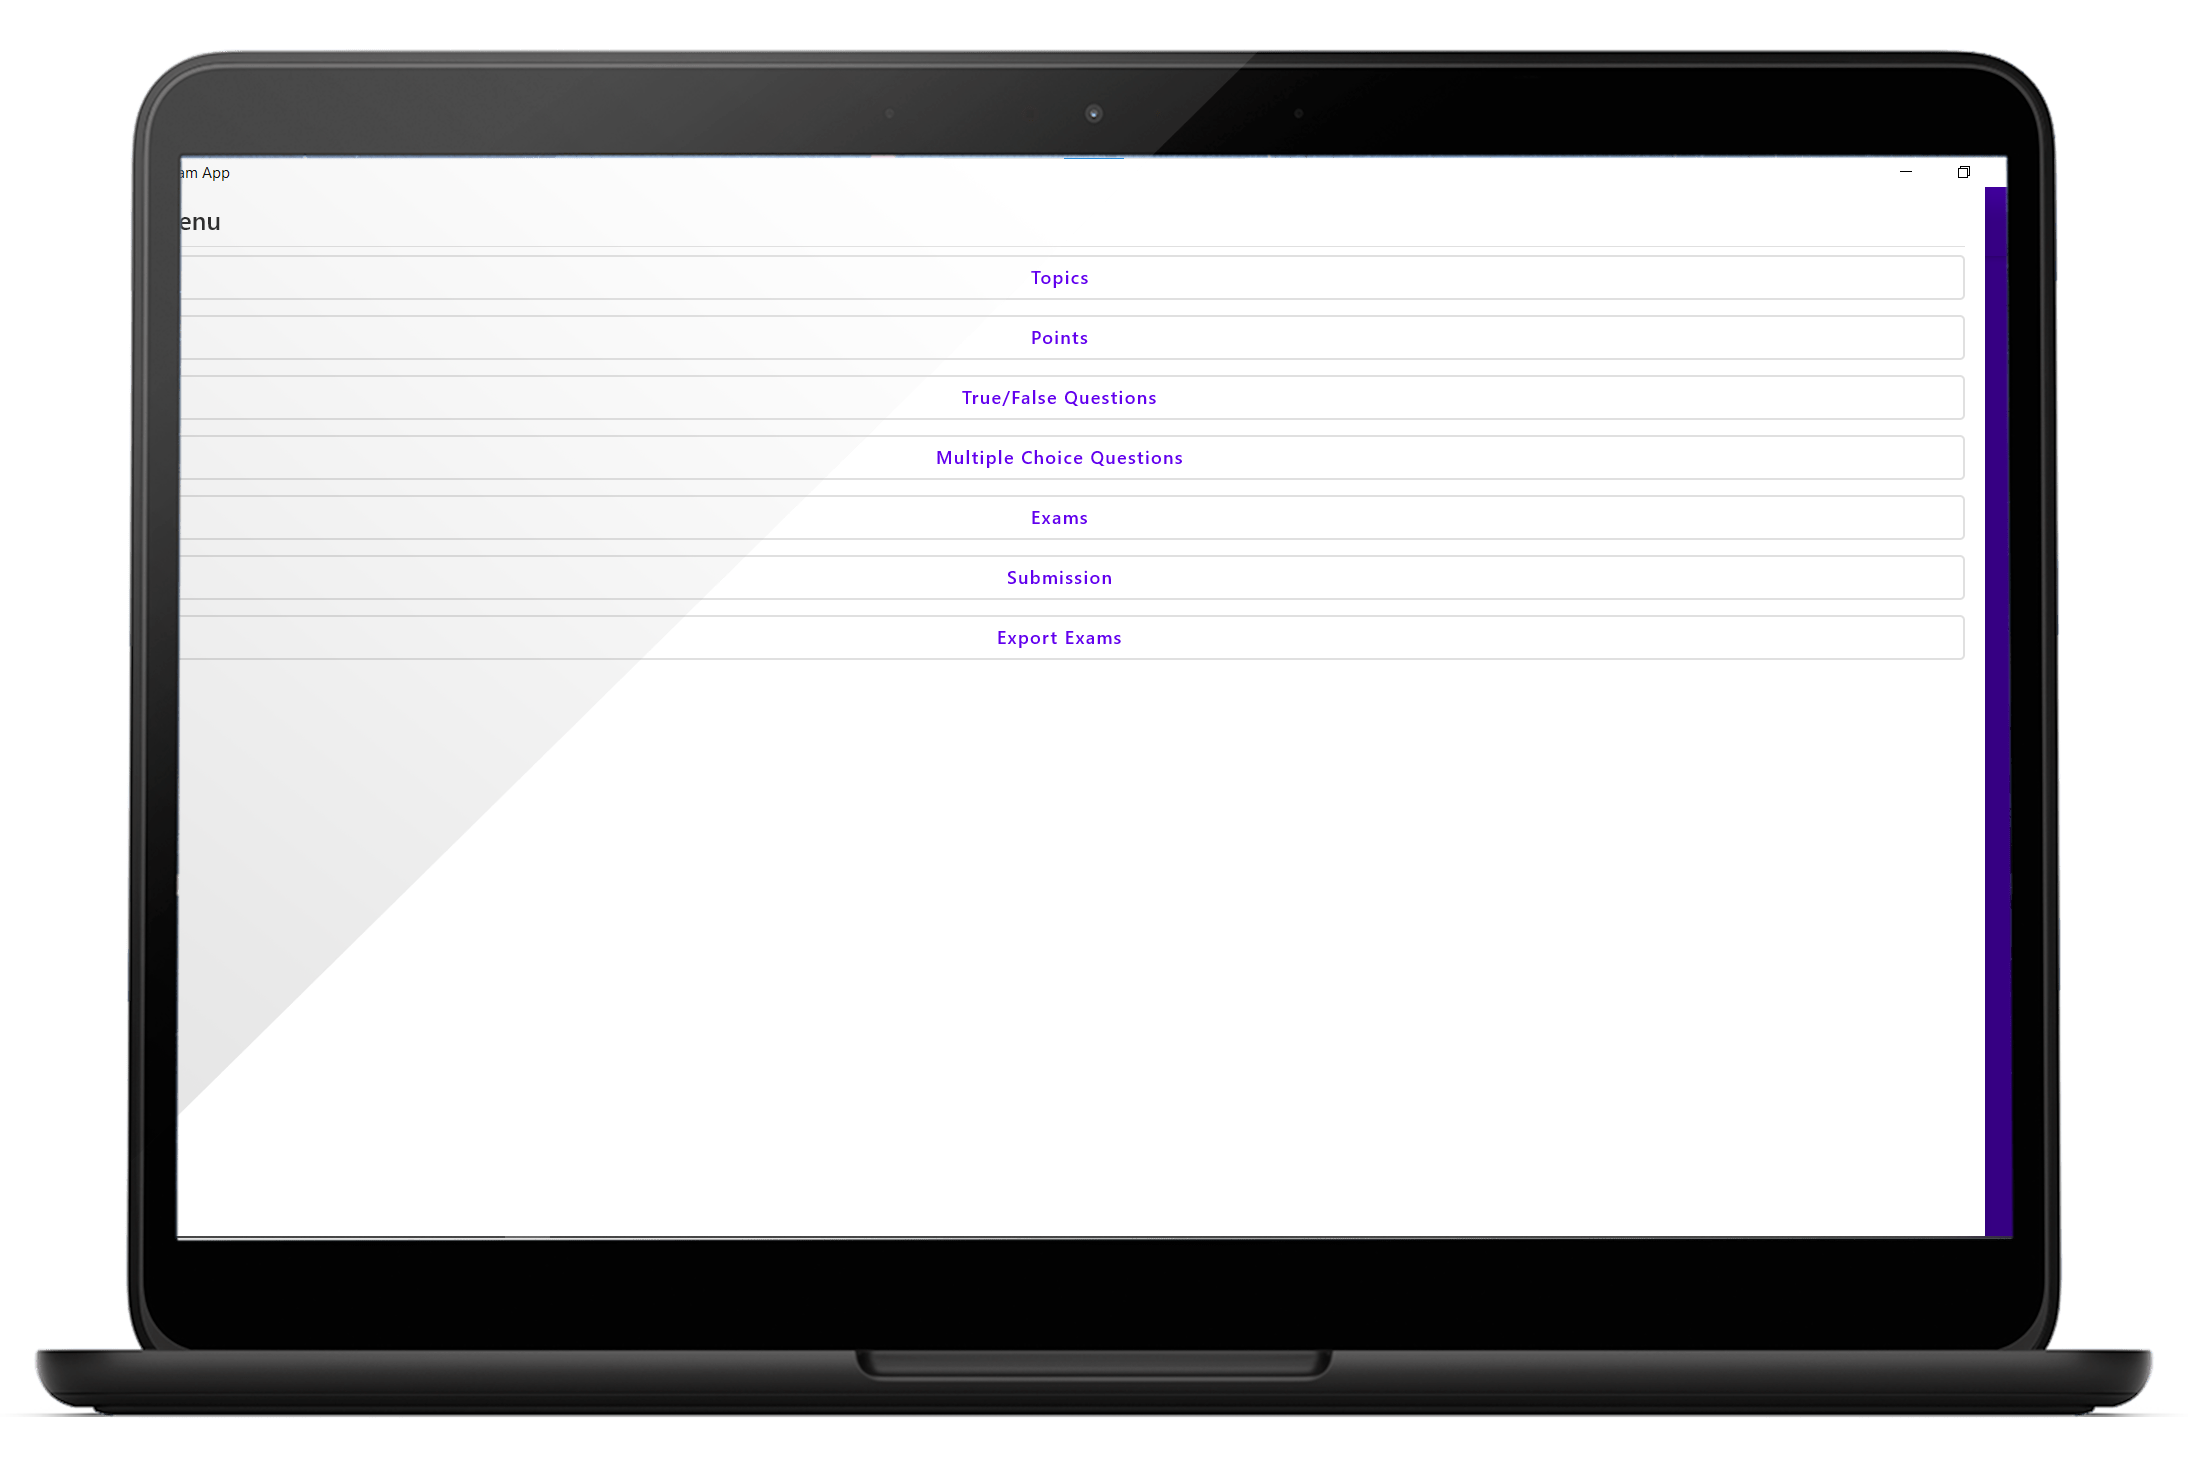
\includegraphics[width=0.5\textwidth, keepaspectratio]{figures/MainScreen_Desktop2_framed.png}
    \caption{Kinyitott menüsáv kinézete az asztali alkalmazáson}
    \label{fig:OpenMenu}
\end{figure}

\begin{figure}[!ht]
    \centering
    \begin{tabular}{cc}
        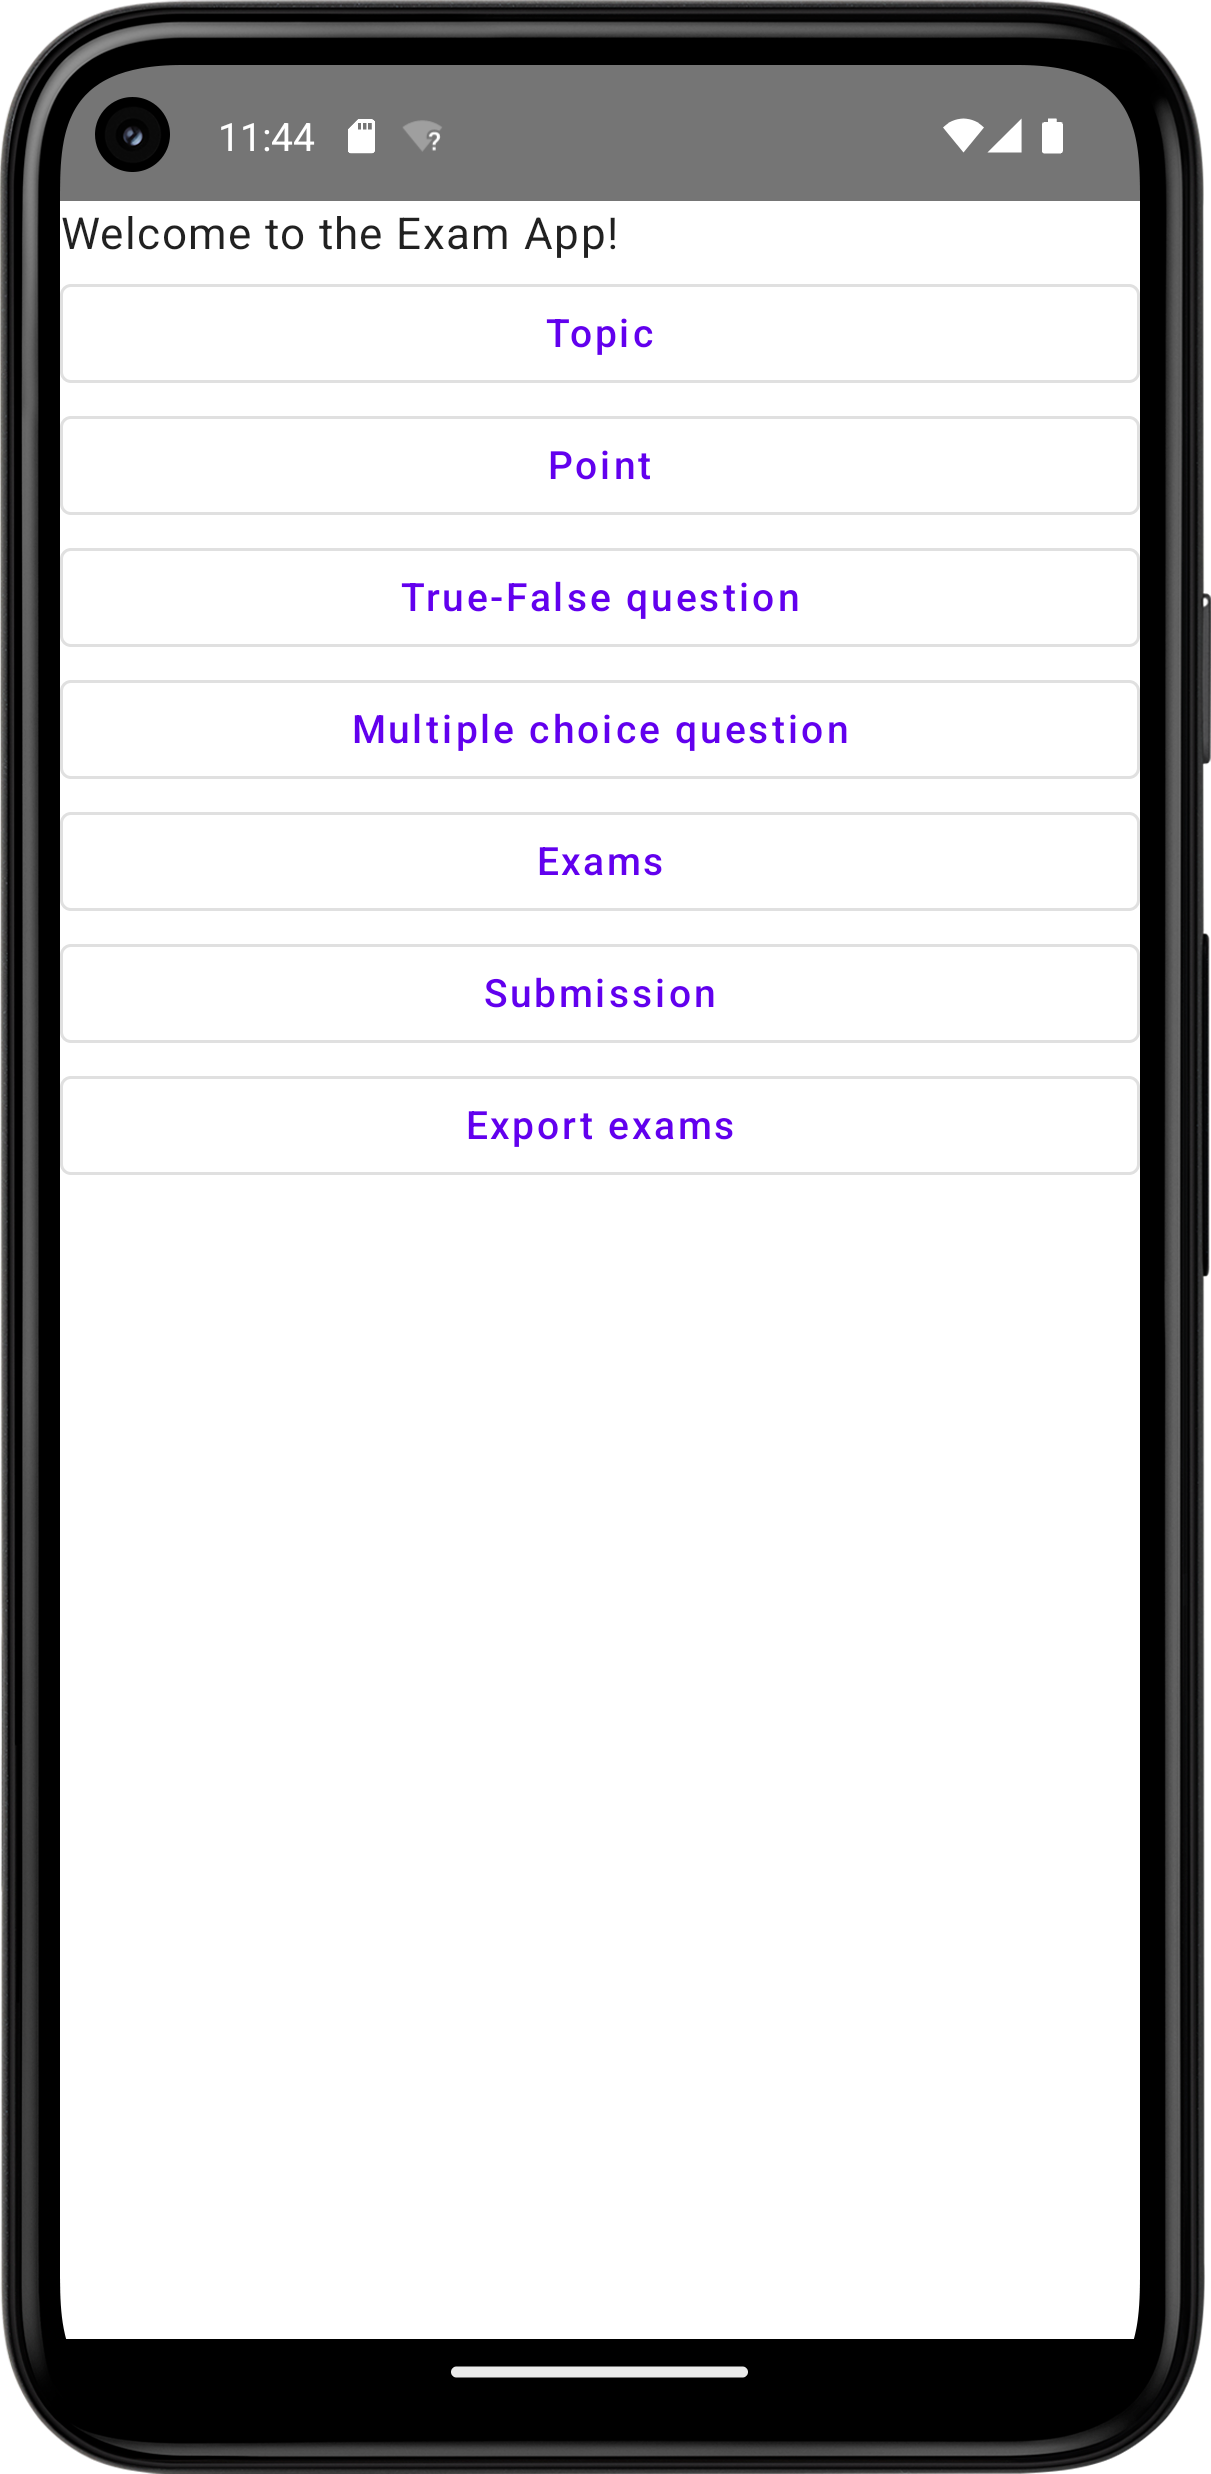
\includegraphics[width=0.3\textwidth, keepaspectratio]{figures/MainScreen_Android.png} & 
        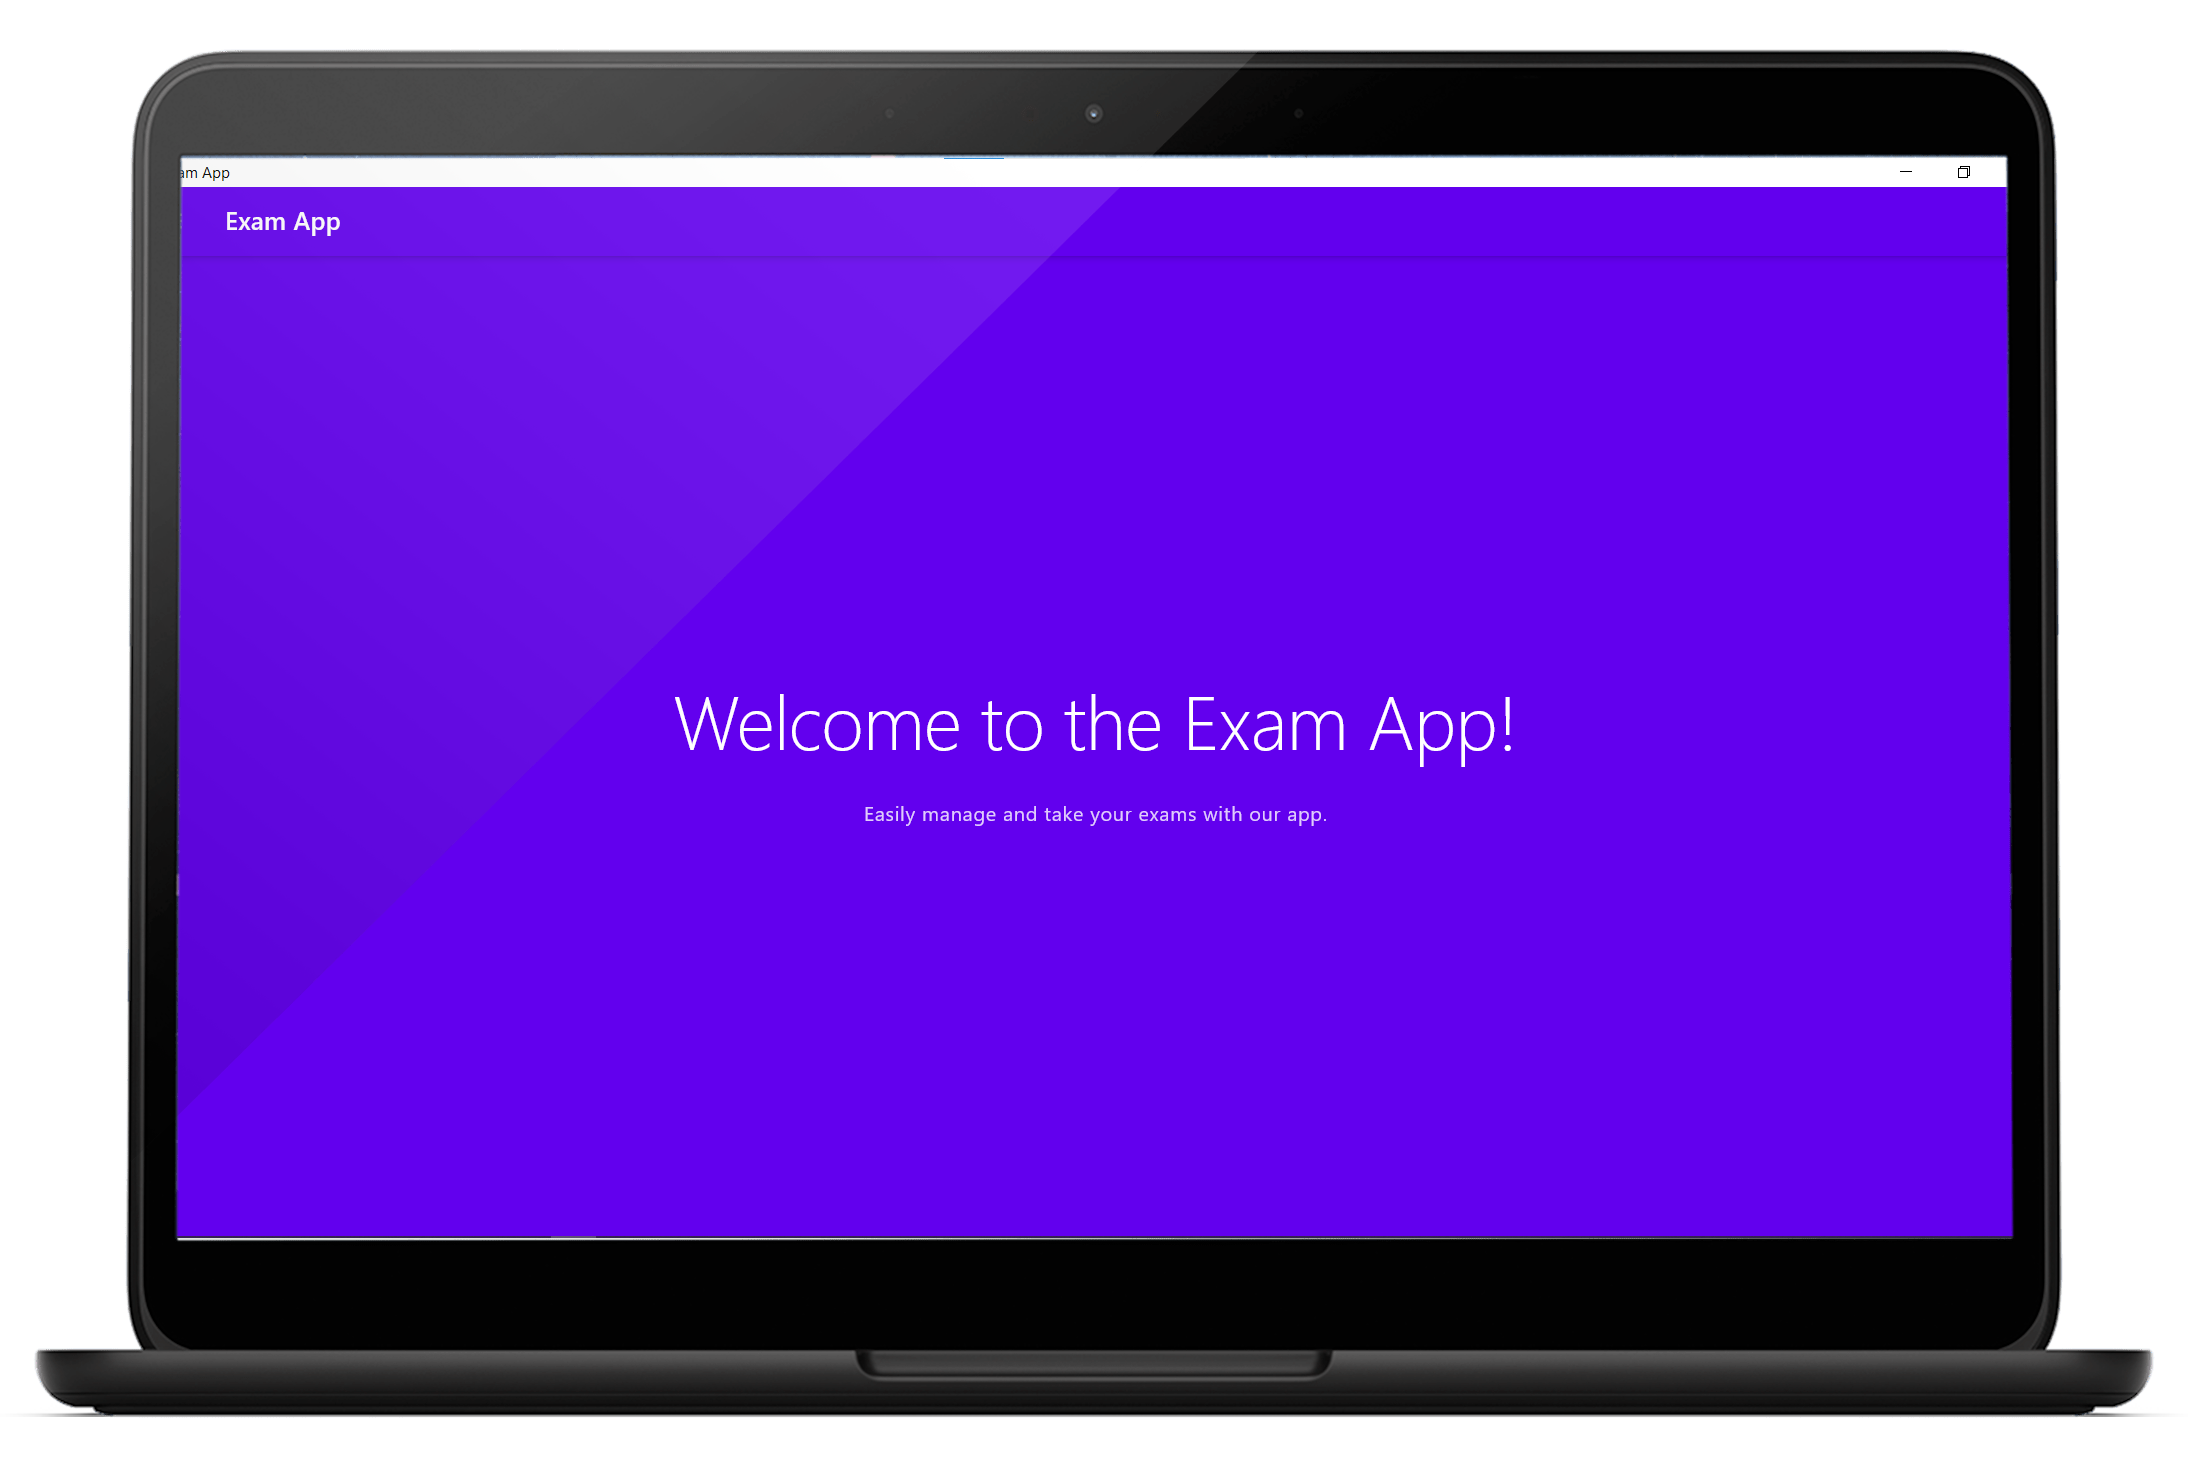
\includegraphics[width=0.5\textwidth, keepaspectratio]{figures/MainScreen_Desktop1_framed.png}
    \end{tabular}
    \caption{A fő képernyő Android és asztali alkalmazáson}
    \label{fig:MainScreen}
\end{figure}


\pagebreak

\subsubsection{Elemek listázása}

Az elemek felsorolásáért egy LazyColumn felel. (\ref{lst:ListScreen}.~kódrészet)
Ez egy előre létrehozott, beépített Composable függvéy.
Több hasznos tulajdonsággal rendelkezik. Alapértelmezett módon görgethetővé válik, ha több elem van benne, mint amennyi kifér egy képernyőre. (\refstruc{fig:ListScreen})
Alkalmas nagyon sok, akár végtelen elem megjelenítésére, bár ehhez szükség van az adtaok ügyes betöltésére is. 
Mindig csak annyi elemet renderel ki amennyi éppen szükséges, látszódik. Előtte és utána van egy kis tartalék puffer, így görgetés esetén nem kell várni az új adtaok betöltésére.
Az elemek testre is szabhatók benne, tökéltes alaklmaási területe lehet egy chat alkalmazás, ahol az elemeket az üzenet küldője alapján lehet színezni.

Ezen a képrenyőn is a Scaffold megoldást választottam így kényelemsen elfér egy navigációs sáv és egy Folating Action Button az új elemek felvételéhez.
Ezeken túl több korábban is bemutaott elem megjelenik ebben a kódrészletben is.
Ahogy látszik az alábbi kódrészetben is, attól függően lehet elemeket beállítani, hogy milyen feltételhet kötjöük az elemek megjelnítését.
\begin{lstlisting}[caption={Listázó képernyő.}, label={lst:ListScreen}, language=Kotlin]
@Composable
fun MultipleChoiceQuestionListResultScreen(
    ...
) {
    Scaffold(
        topBar = { TopAppBarContent(stringResource(Res.string.multiple_choice_question_list), navigateBack) },
        floatingActionButton = {
            FloatingActionButton(
                onClick = { addNewQuestion() }, ...
            ) {Icon(Icons.Filled.Add, contentDescription = "Add") }
        }
    ) { padding ->
        LazyColumn(
            contentPadding = padding,
            ...
        ) {
            if (questions.isEmpty()) {
                item { Box(modifier = Modifier ...) { Text(...) } }
            } else {
                items(questions) { question ->
                    TextButton(
                        onClick = { navigateToMultipleChoiceQuestionDetails(question.uuid) },
                        modifier = Modifier ...
                    ) {
                        Text(text = question.name, ...)
}}}}}}
\end{lstlisting}

\begin{figure}[!ht]
    \centering
    \begin{tabular}{cc}
        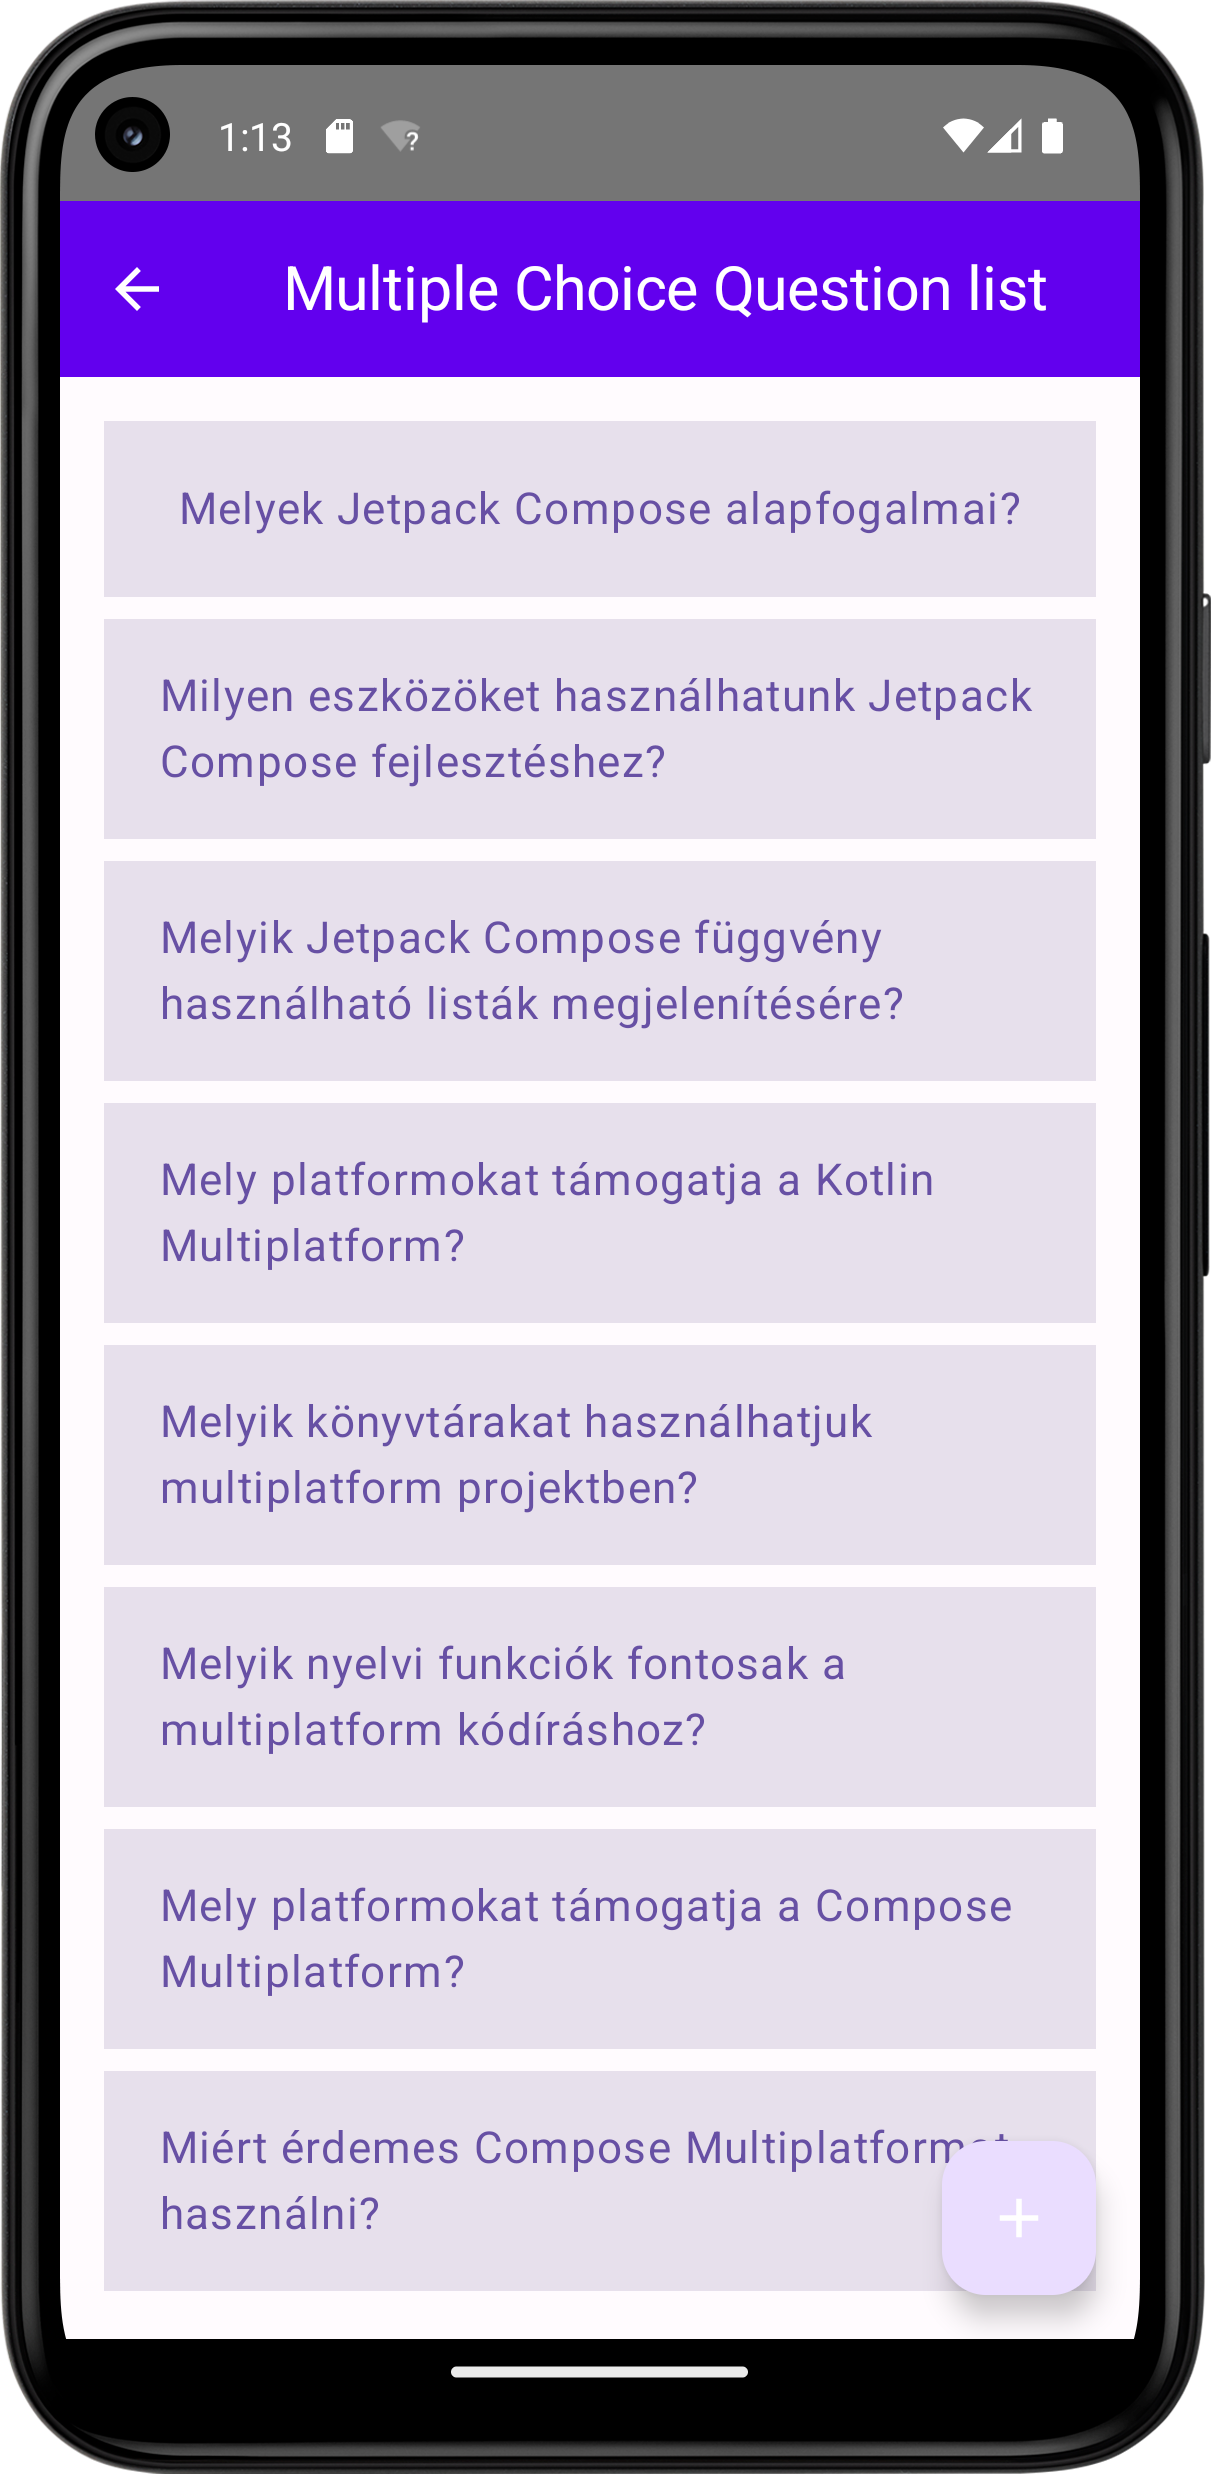
\includegraphics[width=0.3\textwidth, keepaspectratio]{figures/List_Android.png} & 
        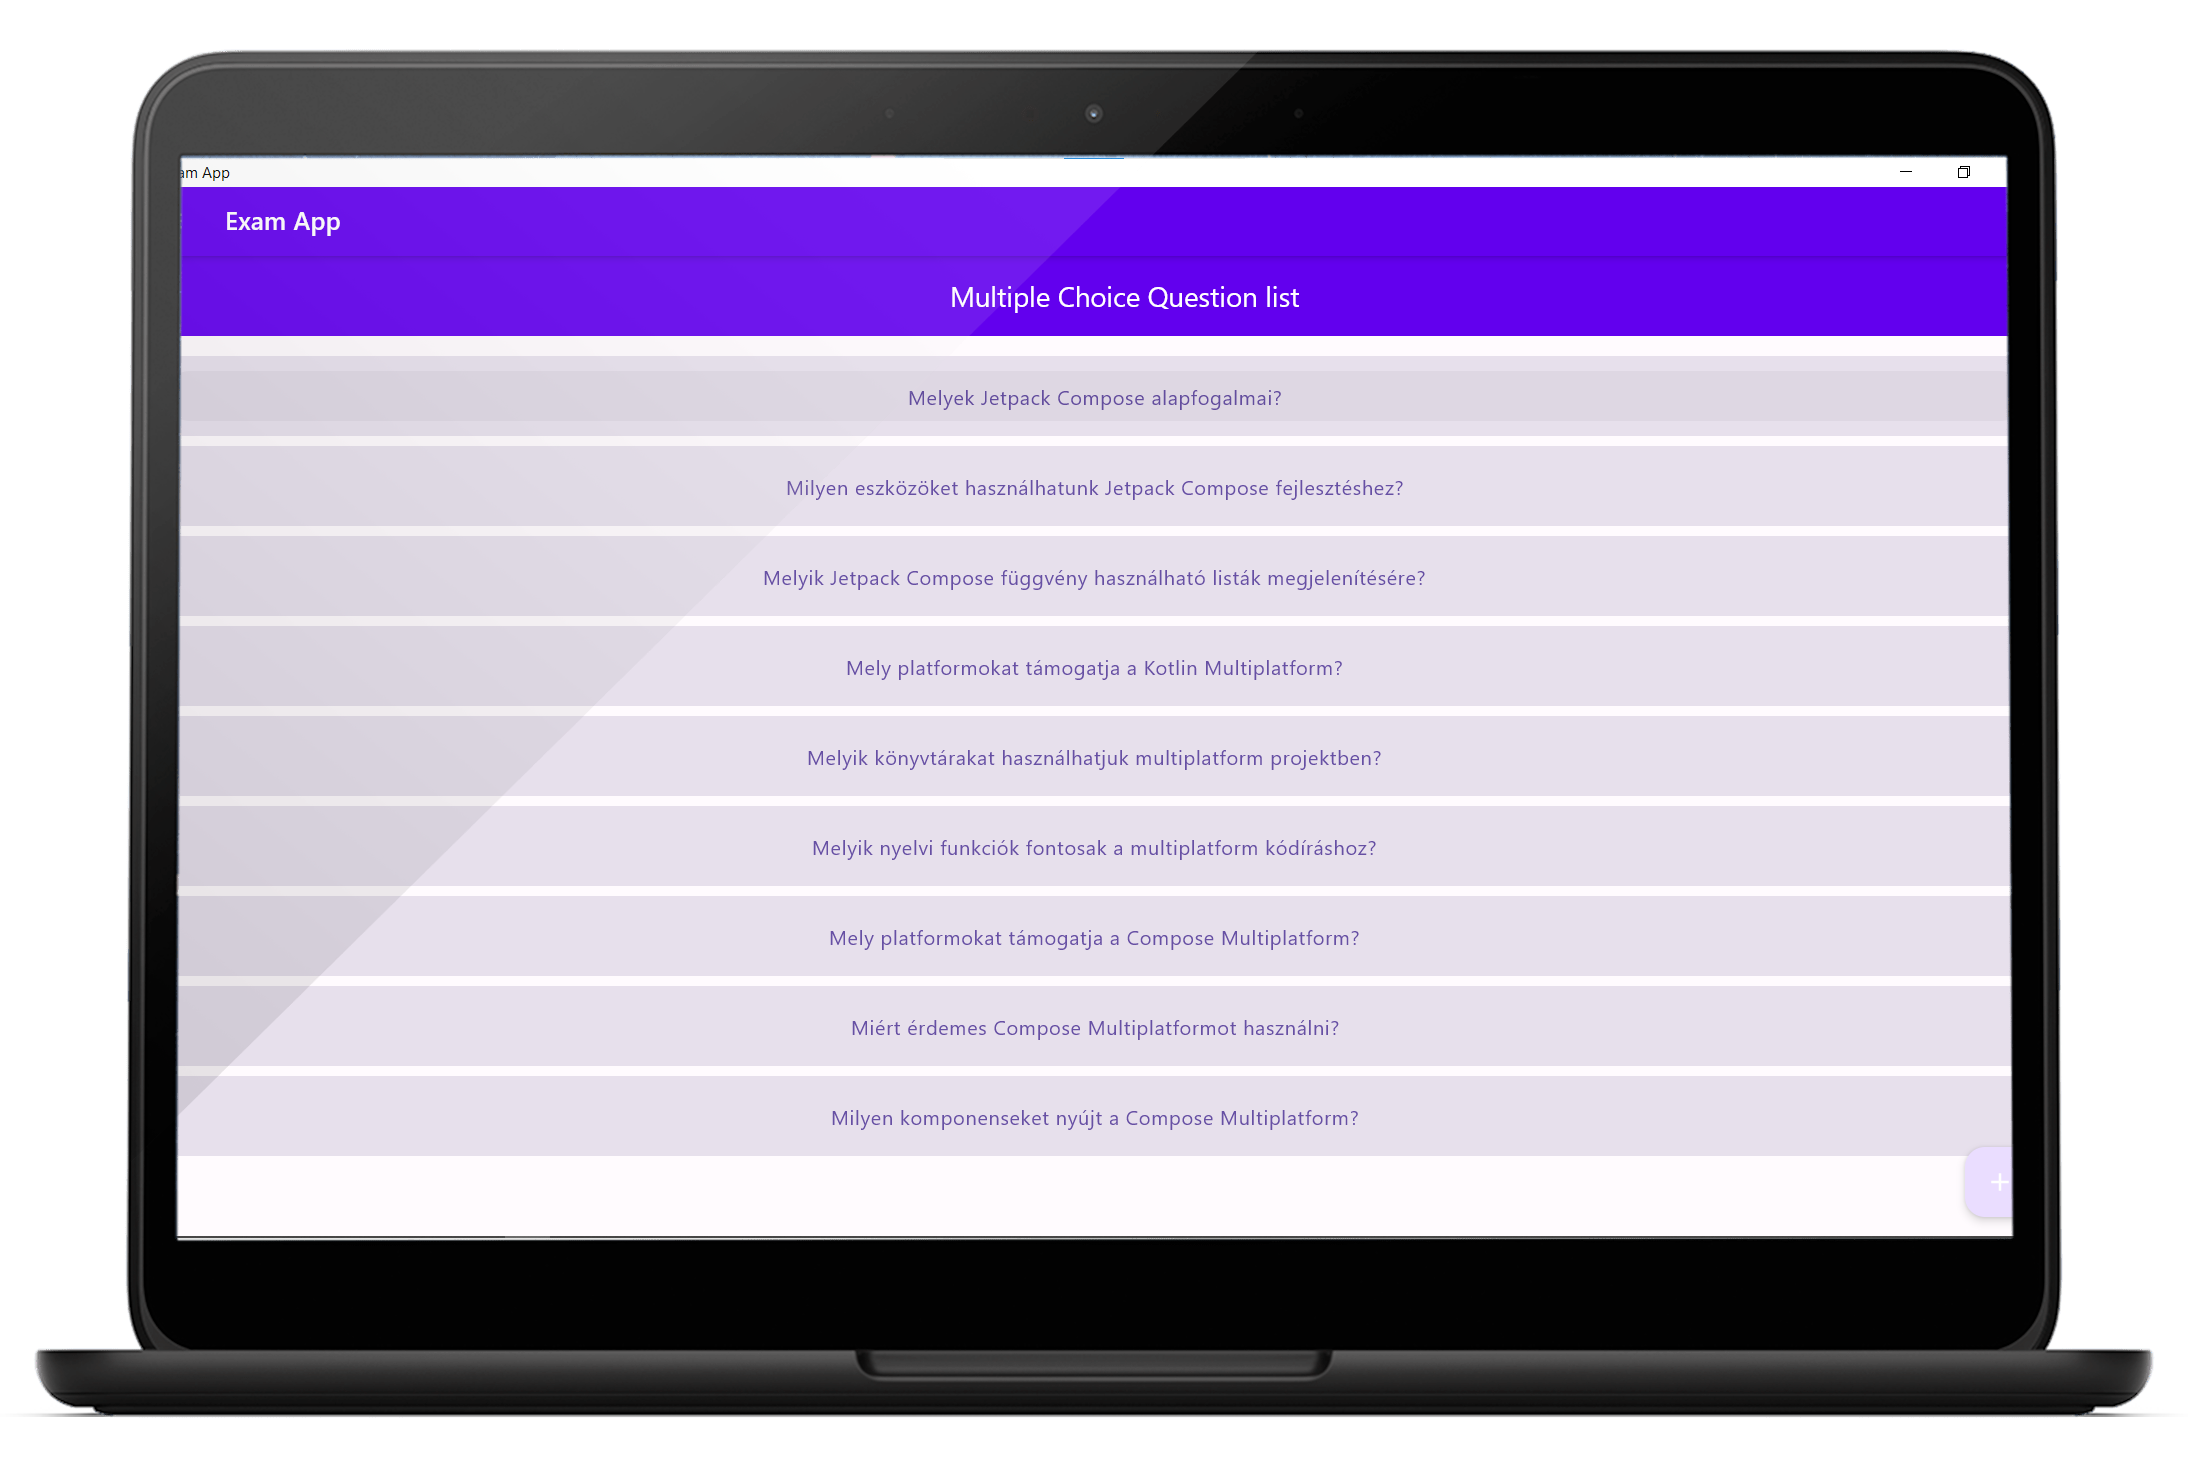
\includegraphics[width=0.6\textwidth, keepaspectratio]{figures/ListView_Desktop_framed.png}
    \end{tabular}
    \caption{A fő képernyő Android és asztali alkalmazáson}
    \label{fig:ListScreen}
\end{figure}


\subsubsection{Részletes nézet}

A részletes oldalak általában csak az összes adatot felsorolják és mutatják meg a felhasználónak.
Ezen kívül tartalmaznak egy törlés opciót ami egy megerősítő ablakot dob fel, mivel a törlés az végleges.
Továbbá innen mehetünk át a szerkesztő oldalra is.

A \refstruc{fig:DetailsScreen} egy érdekesebb megoldást mutat be.
Az oldal tetején a szokásos navigációs sávon kívül elhelyezkedik egy a kérdések közötti keresést segítő rész.
Szűrhetünk kérdéstíusokra, ezt a csúszka segítségével tehetjük meg, ez egyúttal át is színezi azt a könnyebb megkülönböztethetőség kedvéért.
Ezen kívül szűrhetünk témákra is.
Az utolsó dropdwon menü segítségével választhatunk ki egy kérdést amit a gombbal hozzá adhatunk a listához.

A lista része szintén LazyColumn alapú, itt a kérdések típusa alapjén vannak színezve az elemek.
A kérdésekre kattintva lenyílnak és megnézhetjük a legfontosabb adataikat, és innen is lehet törölni a kérdéseket a listából. Ezzel csak a számonkérésből törlődnek, nem a teljes adatbázsiból.
Hosszan lenyomva az elemet elhúzhatjuk felfelé és lefelé ezzel szabadon átrendzhetjük az kérdések sorrendjét.

\begin{lstlisting}[caption={Kinyitható kérdés megvalósítása.}, label={lst:DetailsScreen}, language=Kotlin]
@Composable
fun ExpandableQuestionItem(...){
    var expandedState by remember { mutableStateOf(false) }
    val rotationState by animateFloatAsState(
        targetValue = if (expandedState) 180f else 0f, label = ""
    )
    val coroutineScope = rememberCoroutineScope()
    Card(
        modifier = Modifier.fillMaxWidth()
            .animateContentSize(
                animationSpec = tween(
                    durationMillis = 300,
                    easing = LinearOutSlowInEasing)),
        onClick = { expandedState = !expandedState}
    ) {
        Row(modifier = Modifier.background(if(question.typeOrdinal == Type.trueFalseQuestion.ordinal) PaleDogwood else Green)) {
            Column(...) {
                when (question.typeOrdinal) {
                    Type.trueFalseQuestion.ordinal -> {
                        val trueFalseQuestion = question as TrueFalseQuestionDto
                        if (expandedState) {
                            TrueFalseQuestionDetails(
                                trueFalseQuestion = trueFalseQuestion.toTrueFalseQuestionDetails(...),
                                modifier = Modifier.fillMaxWidth(),
                                colors = CardDefaults.cardColors(
                                    containerColor = PaleDogwood,
                                    contentColor = Purple40
                                )
                            )
                            RemoveButton(coroutineScope, examViewModel, question)
                        } else {
                            CollapsedQuestion(
                                question = trueFalseQuestion.question,
                                containerColor = PaleDogwood, contentColor = Purple40
                        )}}
                    Type.multipleChoiceQuestion.ordinal -> {...}
                }}
                IconButton(modifier = Modifier.weight(1f).alpha(0.2f).rotate(rotationState),
                    onClick = {expandedState = !expandedState}) {
                    Icon(
                        imageVector = Icons.Default.ArrowDropDown,
                        contentDescription = "Drop-Down Arrow"
                )}
        }}}
\end{lstlisting}

A fenti kódrészletben sok érdekes megoldás látható.
Az elején felveszünk több Statet, de ezek közül a második a legizgalamsabb. Ez a State lesz az egyik fontos eleme az animációnak.
Felhasználjuk benne az első Statet aminek az állapota a kérdésre kattintáskot változik, és ennek az értéktől függően (nyitott vagy csukott) változtatjuk az animácihóz tartozó értéket.
A Card Composable elemenhasználjuk az animációt, ezt az animateContentSize segítségével tehetjük meg.
Vannak más fajta animációk is,mindegyik testreszabható és sajátok is létrehozhatóak. Ez esetben egy tween animációt használunk ami 0.3 másodperc alatt az összecsukott állpotról egy nyitott állapotra áll át.
Attól változik meg az elem és játszódik le az animáció, hogy rákattintunk a kérdésre.
Mivel a Cardon az animateContentSizet használtuk ezért amikor az expandedState megváltozok akkor a CollapsedQuestion helyett a recomposoition után a TrueFalseQuestionDetails kell megjeleníteni ez méretváltozással jár, ezt követi le az animáció ezáltal nem hirtelen ugrik egyet a képrenyő, hanem lekövethető módon változik meg.
A rotationState pedig az ArrowDropDown elem animálásban játszik szerepet, így az ikont el tudjuk forgatni 180 fokkal, ehhez a Modifierhez tartozó rotate(Int) extension functiont tudjuk használni.

\begin{figure}[!ht]
    \centering
    \begin{tabular}{cc}
        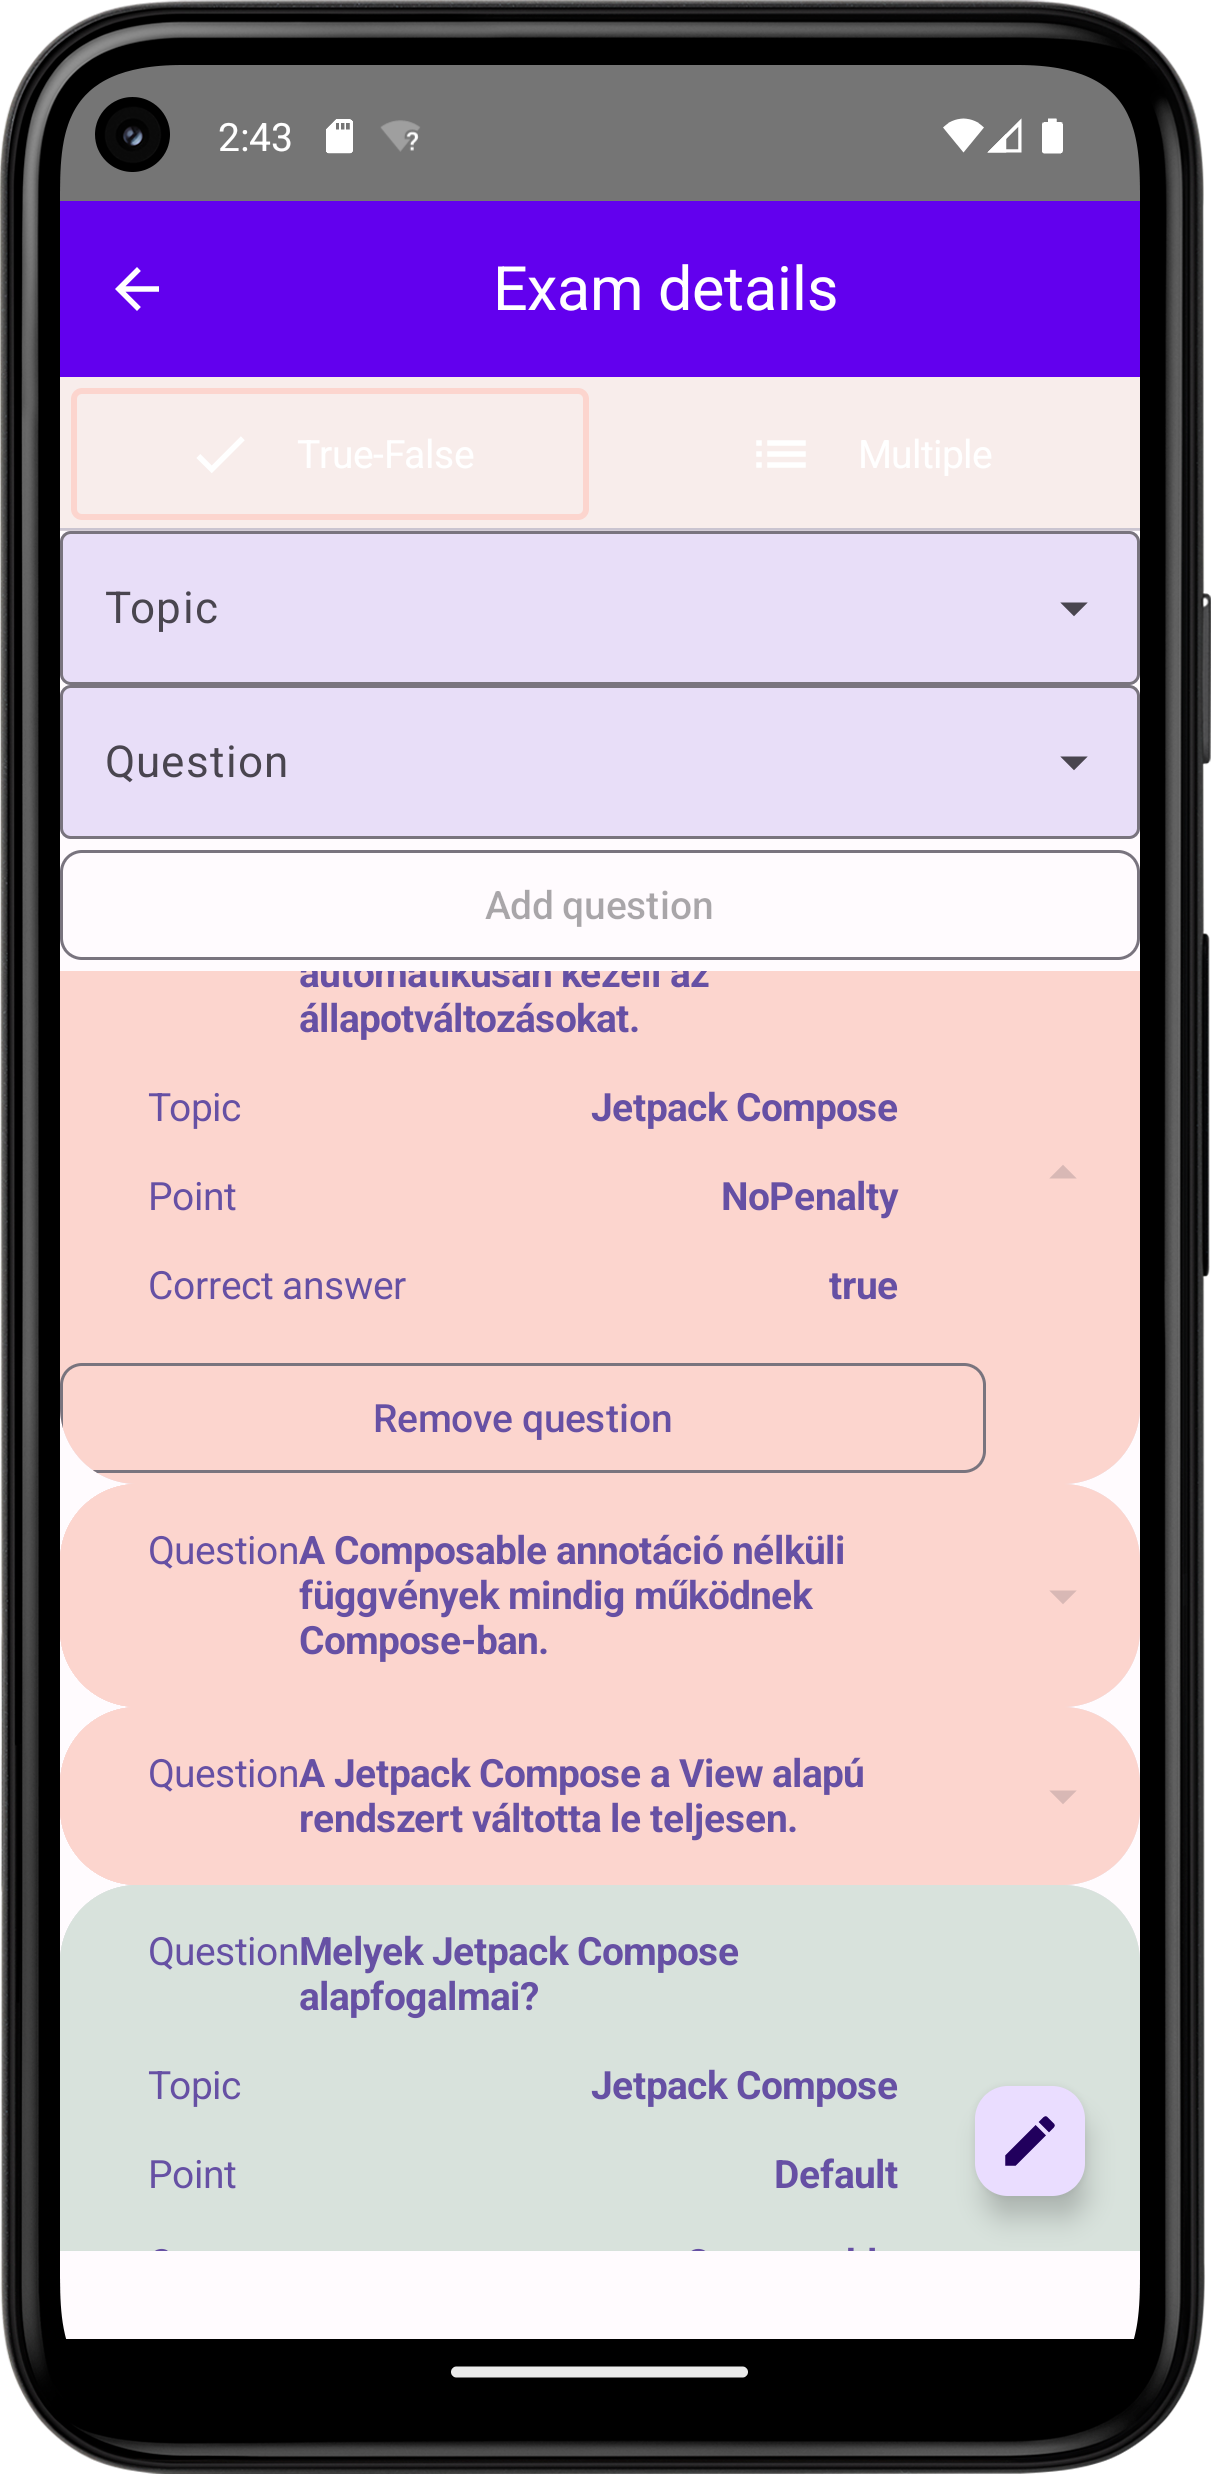
\includegraphics[width=0.3\textwidth, keepaspectratio]{figures/Details_Android.png} & 
        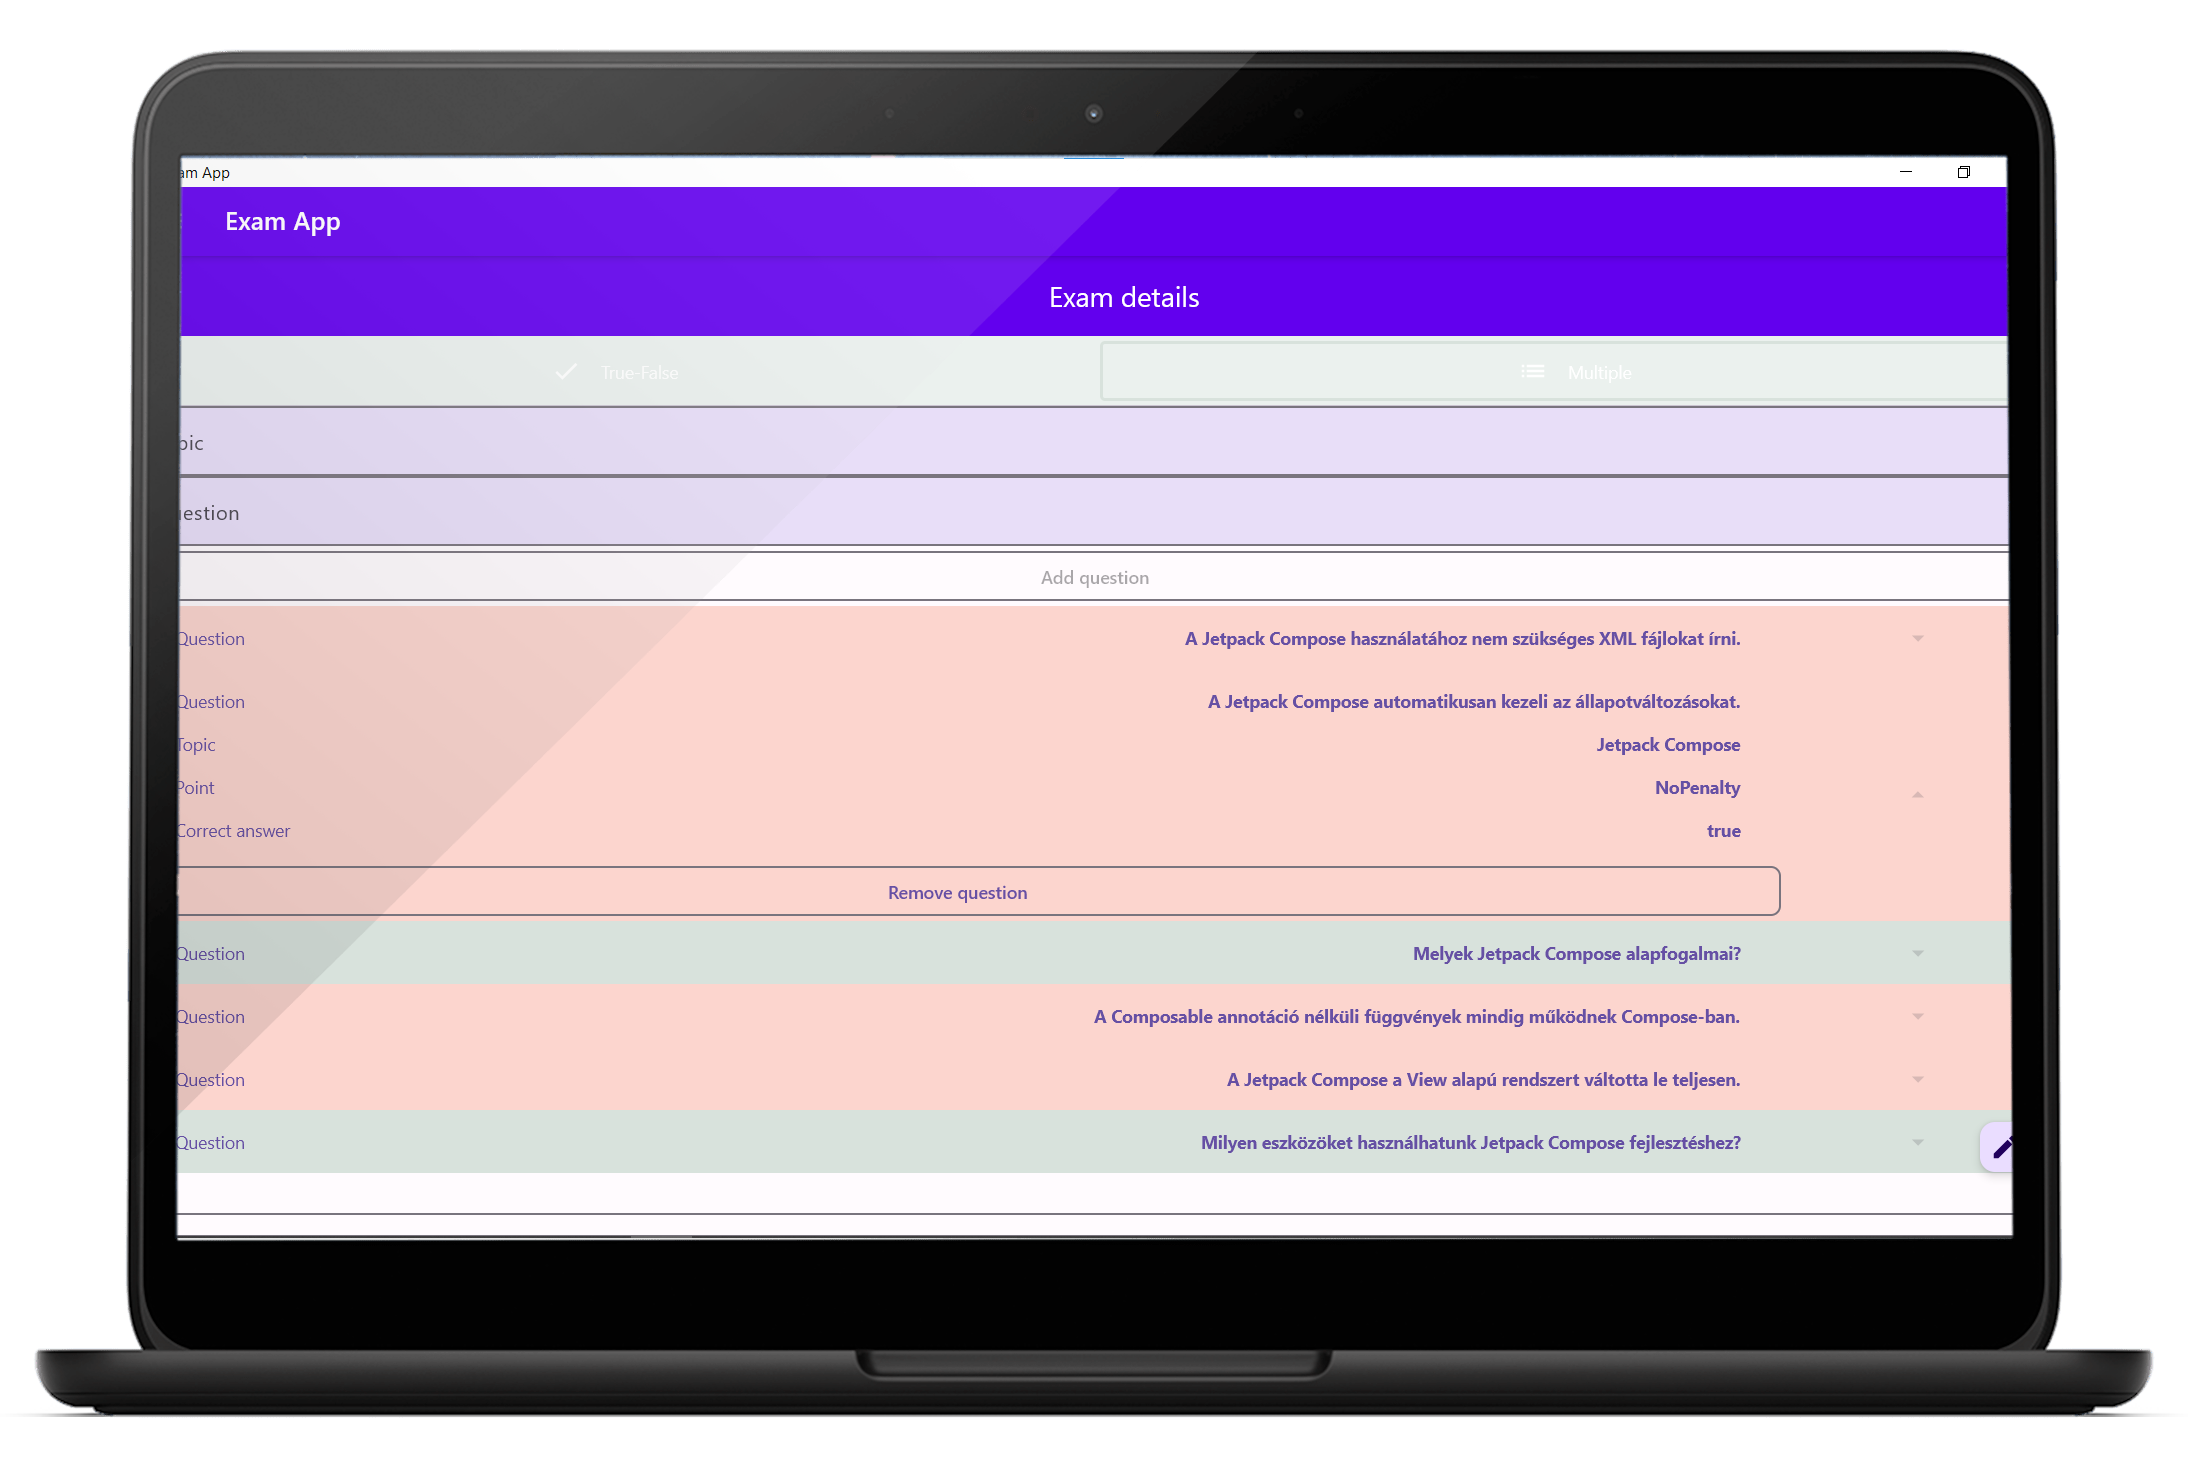
\includegraphics[width=0.6\textwidth, keepaspectratio]{figures/Details_Desktop_framed.png}
    \end{tabular}
    \caption{Egy érdekesebb részletes képernyő, a vizsgák összeállításához tartozik.}
    \label{fig:DetailsScreen}
\end{figure}

\section{Navigáció}


\section{ViewModel}


\section{HTTP kliens}


\section{PDF}


\section{Szöveg felismerés}
